\documentclass[12pt,fleqn]{article}\usepackage{../common}
\begin{document}
En Yakin k-Komsu (k-Nearest Neighbor)

Yapay Ogrenim alaninda ornek bazli ogrenen algoritmalardan bilinen kNN,
egitim verinin kendisini siniflama (classification) amacli olarak kullanir,
yeni bir model ortaya cikartmaz. Algoritma soyle isler: etiketleri bilinen
egitim verisi alinir ve bir kenarda tutulur. Yeni bir veri noktasi
gorulunce bu veriye geri donulur ve o noktaya ``en yakin'' k tane nokta
bulunur. Daha sonra bu noktalarin etiketlerine bakilir ve cogunlugun
etiketi ne ise, o etiket yeni noktanin etiketi olarak kabul edilir.

``En yakin'' sozu bir kordinat sistemi anlamina geliyor, ve kNN, aynen
k-Means ve diger pek cok kordinatsal ogrenme yontemi gibi eldeki cok
boyutlu veri noktalarinin elemanlarini bir kordinat sistemindeymis gibi
gorur. Kiyasla mesela APriori gibi bir algoritma metin bazli veriyle oldugu
gibi calisabilirdi.

Peki arama baglaminda, bir veri obegi icinden en yakin noktalari bulmanin
en basit yolu nedir? Listeyi bastan sonra taramak (kaba kuvvet yontemi
-brute force-) ve her listedeki nokta ile yeni nokta arasindaki mesafeyi
teker teker hesaplayip en yakin k taneyi icinden secmek bir yontem. Bu
basit algoritmanin yuku $O(N)$'dir. 

Fakat bu islemi daha hizli yapmak mumkun. 

Arama algoritmalari kullanarak egitim verilerini bir agac yapisi uzerinden
arayarak erisim hizini $O(\log N)$'e indirmek mumkundur. 

Kuresel Agaclar (Ball Tree) 

Diyelim ki elimide iki boyutlu uzayda alttaki gibi bir veri var. 

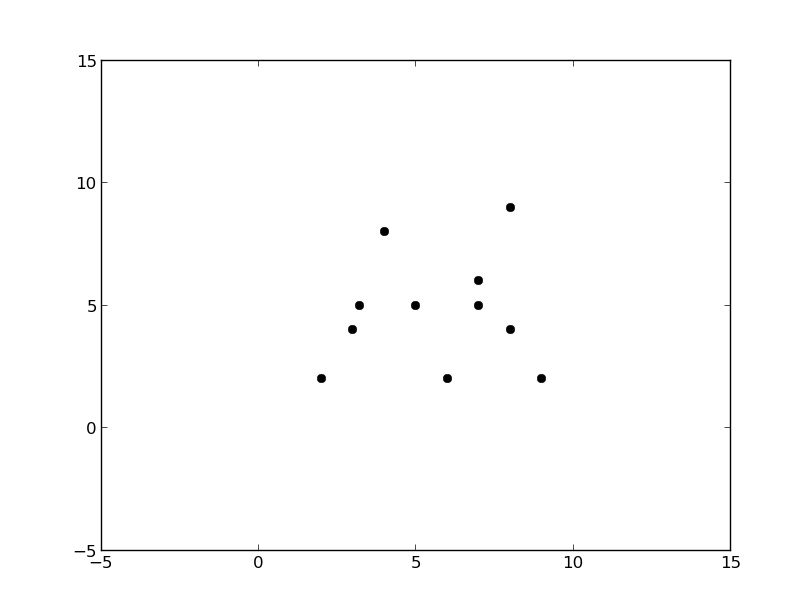
\includegraphics[height=7cm]{knn-main.png}


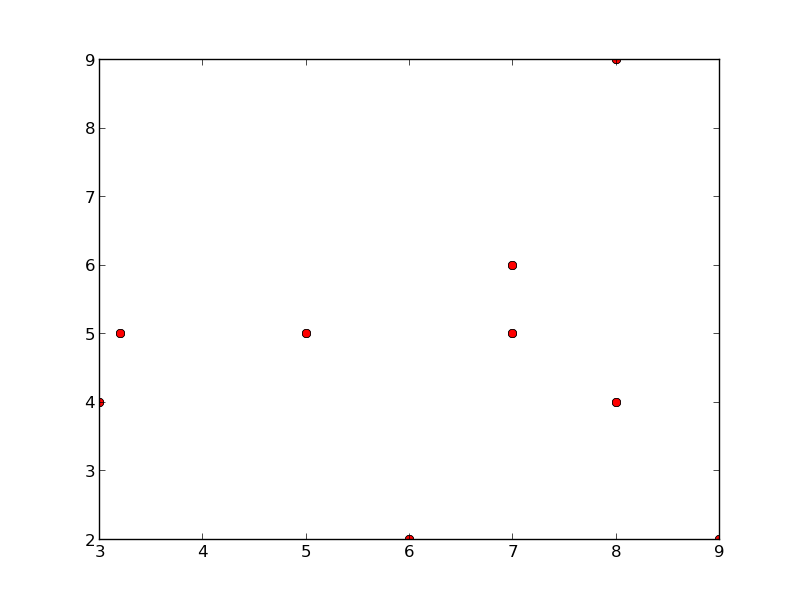
\includegraphics[height=7cm]{knn0.png}

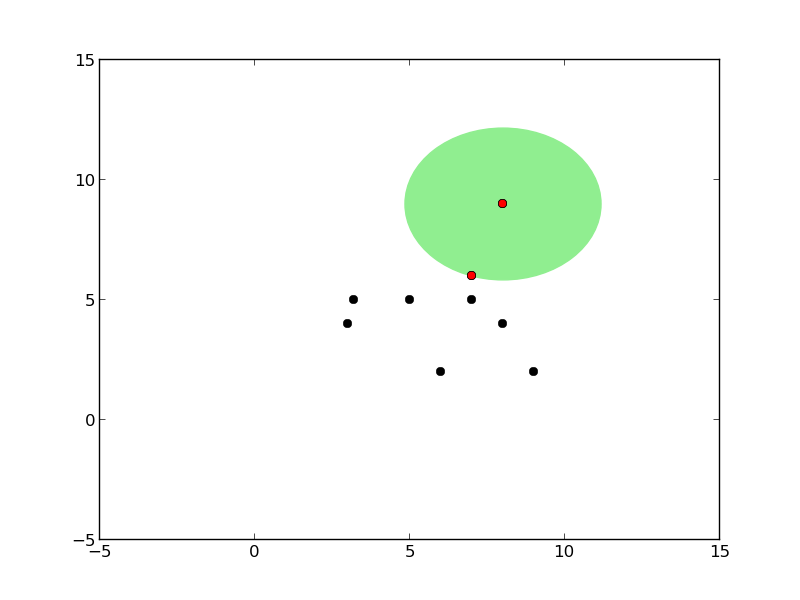
\includegraphics[height=7cm]{knn1.png}

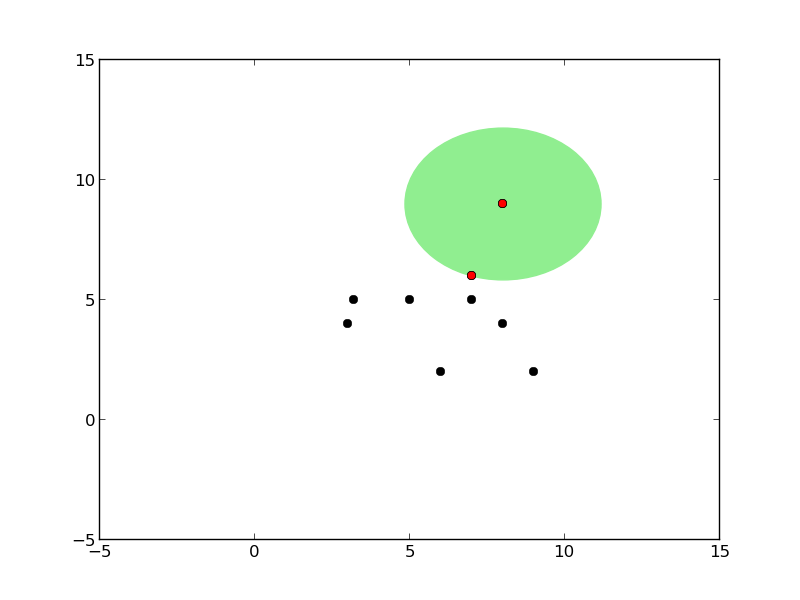
\includegraphics[height=7cm]{knn2.png}

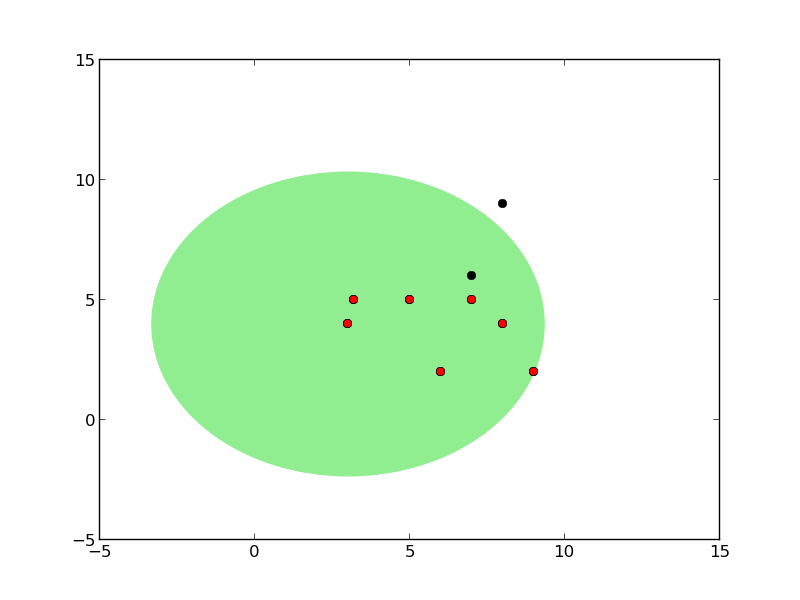
\includegraphics[height=7cm]{knn3.png}

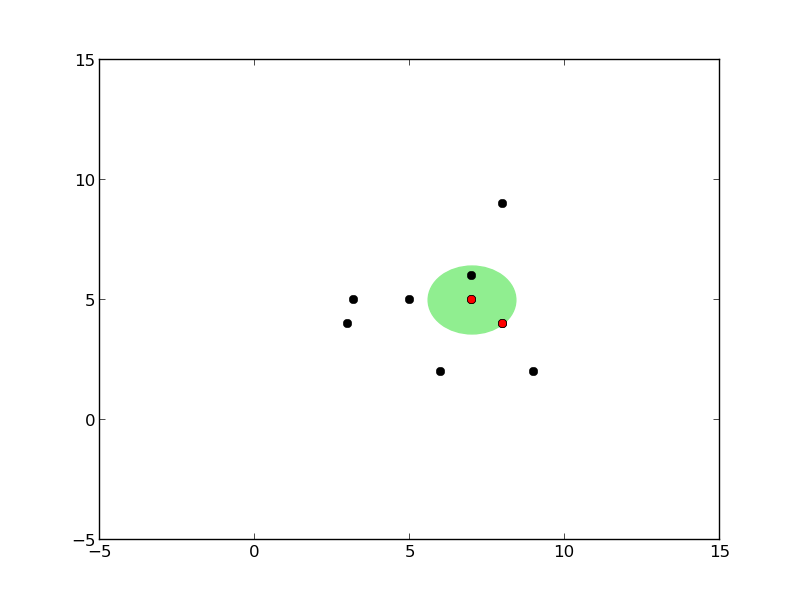
\includegraphics[height=7cm]{knn4.png}

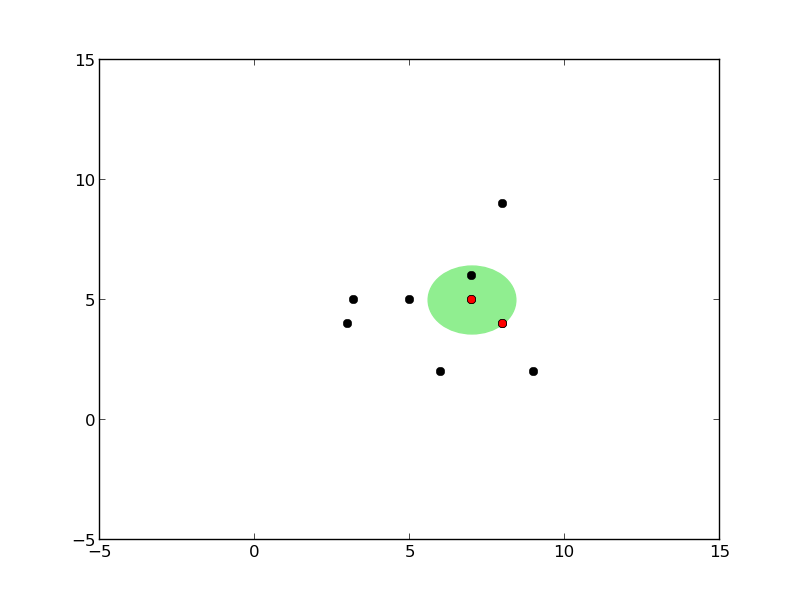
\includegraphics[height=7cm]{knn5.png}

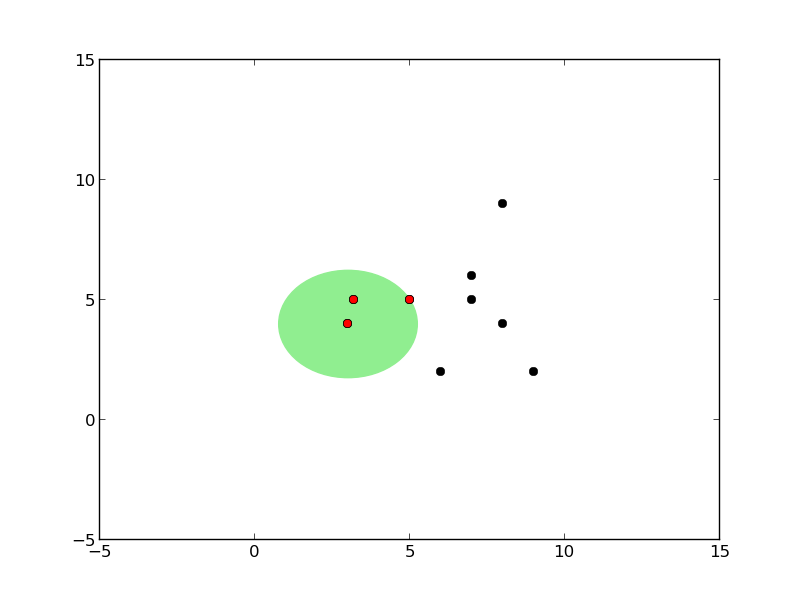
\includegraphics[height=7cm]{knn6.png}

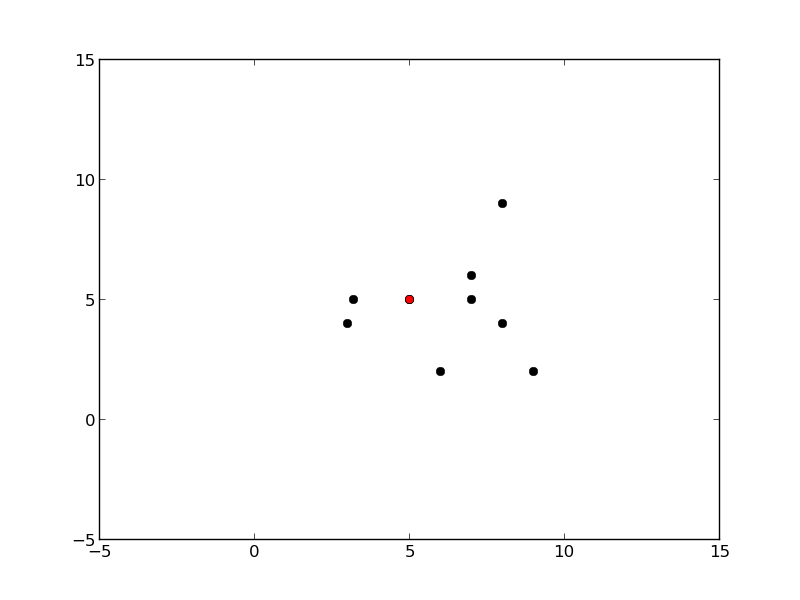
\includegraphics[height=7cm]{knn7.png}

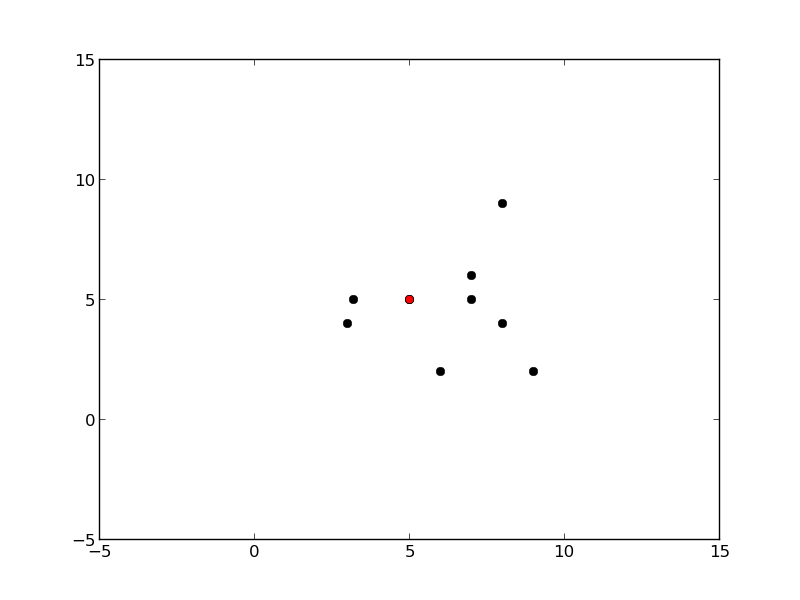
\includegraphics[height=7cm]{knn8.png}



\end{document}
